\documentclass{standalone}
\usepackage[T1]{fontenc}
\usepackage{textcomp}

\usepackage{ifluatex,ifxetex}
\ifluatex
  \usepackage{fontspec}
  \setmainfont{Free Serif}
\else\ifxetex
  \usepackage{fontspec}
  \setmainfont{FreeSerif}
\else
  \usepackage{ucs}
  \SetUnicodeOption{mathletters}
  \usepackage[utf8x]{inputenc}
\fi\fi

\usepackage{gnuplot-lua-tikz}
\pagestyle{empty}
\usepackage[active,tightpage]{preview}
\PreviewEnvironment{tikzpicture}
\setlength\PreviewBorder{\gpbboxborder}
\begin{document}
\large
\begin{tikzpicture}[gnuplot]
\node at (5.84,4.7) {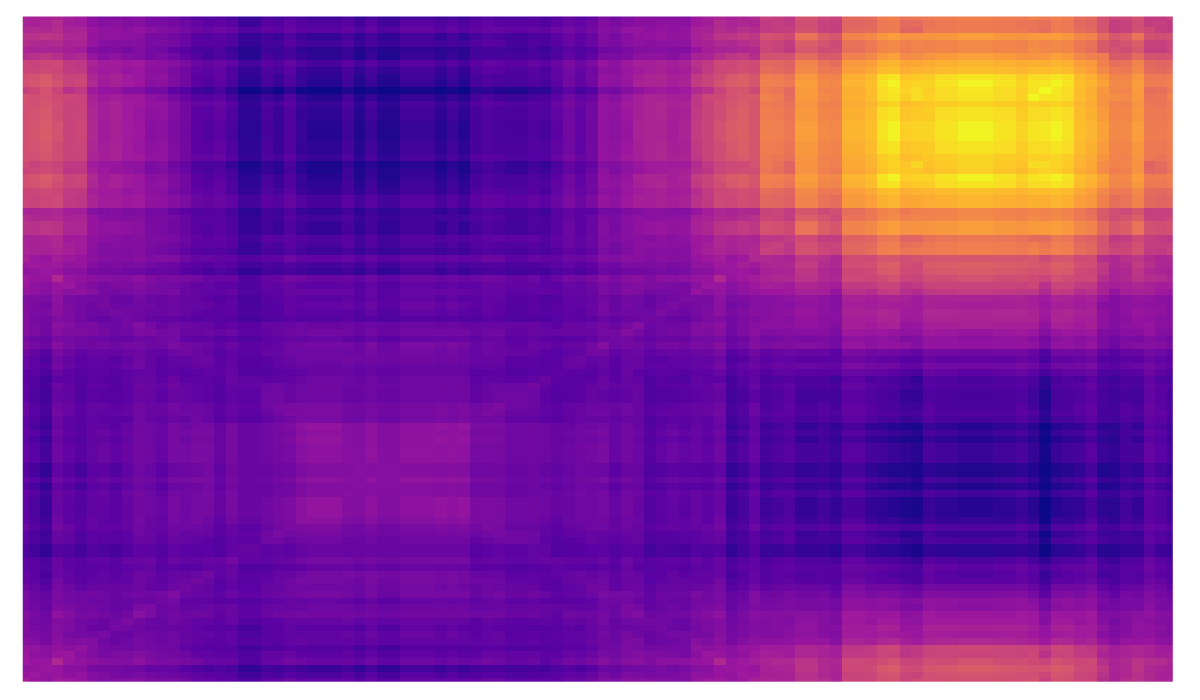
\includegraphics[width=3.69in,height=3.09in]{cov-naked.png}};
%% generated with GNUPLOT 6.0p4 (Lua 5.4; terminal rev. Jun 2020, script rev. 120)
%% Sun Jul  5 22:55:32 2026
%\path (0.000,0.000) rectangle (12.500,8.750);
\gpcolor{color=gp lt color border}
\gpsetlinetype{gp lt border}
\gpsetdashtype{gp dt solid}
\gpsetlinewidth{2.00}
\draw[gp path] (1.320,0.985)--(1.500,0.985);
\draw[gp path] (10.313,0.985)--(10.133,0.985);
\node[gp node right] at (1.136,0.985) {$1$};
\draw[gp path] (1.320,2.416)--(1.500,2.416);
\draw[gp path] (10.313,2.416)--(10.133,2.416);
\node[gp node right] at (1.136,2.416) {$20$};
\draw[gp path] (1.320,3.922)--(1.500,3.922);
\draw[gp path] (10.313,3.922)--(10.133,3.922);
\node[gp node right] at (1.136,3.922) {$40$};
\draw[gp path] (1.320,5.428)--(1.500,5.428);
\draw[gp path] (10.313,5.428)--(10.133,5.428);
\node[gp node right] at (1.136,5.428) {$60$};
\draw[gp path] (1.320,6.935)--(1.500,6.935);
\draw[gp path] (10.313,6.935)--(10.133,6.935);
\node[gp node right] at (1.136,6.935) {$80$};
\draw[gp path] (1.320,8.441)--(1.500,8.441);
\draw[gp path] (10.313,8.441)--(10.133,8.441);
\node[gp node right] at (1.136,8.441) {$100$};
\draw[gp path] (1.320,0.985)--(1.320,1.165);
\draw[gp path] (1.320,8.441)--(1.320,8.261);
\node[gp node center] at (1.320,0.677) {$1$};
\draw[gp path] (3.046,0.985)--(3.046,1.165);
\draw[gp path] (3.046,8.441)--(3.046,8.261);
\node[gp node center] at (3.046,0.677) {$20$};
\draw[gp path] (4.863,0.985)--(4.863,1.165);
\draw[gp path] (4.863,8.441)--(4.863,8.261);
\node[gp node center] at (4.863,0.677) {$40$};
\draw[gp path] (6.679,0.985)--(6.679,1.165);
\draw[gp path] (6.679,8.441)--(6.679,8.261);
\node[gp node center] at (6.679,0.677) {$60$};
\draw[gp path] (8.496,0.985)--(8.496,1.165);
\draw[gp path] (8.496,8.441)--(8.496,8.261);
\node[gp node center] at (8.496,0.677) {$80$};
\draw[gp path] (10.313,0.985)--(10.313,1.165);
\draw[gp path] (10.313,8.441)--(10.313,8.261);
\node[gp node center] at (10.313,0.677) {$100$};
\draw[gp path] (1.320,8.441)--(1.320,0.985)--(10.313,0.985)--(10.313,8.441)--cycle;
\draw[gp path] (1.320,8.441)--(1.320,0.985)--(10.313,0.985)--(10.313,8.441)--cycle;
\node[gp node center] at (0.6,4.713) {$i$};
\node[gp node center] at (5.816,0.215) {$j$};
\gpfill{rgb color={0.051,0.031,0.529}} (10.538,0.985)--(10.987,0.985)--(10.987,1.044)--(10.538,1.044)--cycle;
\gpfill{rgb color={0.067,0.030,0.535}} (10.538,1.043)--(10.987,1.043)--(10.987,1.102)--(10.538,1.102)--cycle;
\gpfill{rgb color={0.083,0.029,0.541}} (10.538,1.101)--(10.987,1.101)--(10.987,1.160)--(10.538,1.160)--cycle;
\gpfill{rgb color={0.099,0.028,0.547}} (10.538,1.159)--(10.987,1.159)--(10.987,1.219)--(10.538,1.219)--cycle;
\gpfill{rgb color={0.115,0.026,0.552}} (10.538,1.218)--(10.987,1.218)--(10.987,1.277)--(10.538,1.277)--cycle;
\gpfill{rgb color={0.131,0.025,0.558}} (10.538,1.276)--(10.987,1.276)--(10.987,1.335)--(10.538,1.335)--cycle;
\gpfill{rgb color={0.147,0.024,0.564}} (10.538,1.334)--(10.987,1.334)--(10.987,1.393)--(10.538,1.393)--cycle;
\gpfill{rgb color={0.163,0.023,0.569}} (10.538,1.392)--(10.987,1.392)--(10.987,1.452)--(10.538,1.452)--cycle;
\gpfill{rgb color={0.178,0.022,0.575}} (10.538,1.451)--(10.987,1.451)--(10.987,1.510)--(10.538,1.510)--cycle;
\gpfill{rgb color={0.194,0.020,0.581}} (10.538,1.509)--(10.987,1.509)--(10.987,1.568)--(10.538,1.568)--cycle;
\gpfill{rgb color={0.210,0.019,0.587}} (10.538,1.567)--(10.987,1.567)--(10.987,1.626)--(10.538,1.626)--cycle;
\gpfill{rgb color={0.226,0.018,0.592}} (10.538,1.625)--(10.987,1.625)--(10.987,1.685)--(10.538,1.685)--cycle;
\gpfill{rgb color={0.242,0.017,0.598}} (10.538,1.684)--(10.987,1.684)--(10.987,1.743)--(10.538,1.743)--cycle;
\gpfill{rgb color={0.258,0.015,0.604}} (10.538,1.742)--(10.987,1.742)--(10.987,1.801)--(10.538,1.801)--cycle;
\gpfill{rgb color={0.274,0.014,0.609}} (10.538,1.800)--(10.987,1.800)--(10.987,1.859)--(10.538,1.859)--cycle;
\gpfill{rgb color={0.290,0.013,0.615}} (10.538,1.858)--(10.987,1.858)--(10.987,1.918)--(10.538,1.918)--cycle;
\gpfill{rgb color={0.306,0.012,0.621}} (10.538,1.917)--(10.987,1.917)--(10.987,1.976)--(10.538,1.976)--cycle;
\gpfill{rgb color={0.322,0.011,0.627}} (10.538,1.975)--(10.987,1.975)--(10.987,2.034)--(10.538,2.034)--cycle;
\gpfill{rgb color={0.338,0.009,0.632}} (10.538,2.033)--(10.987,2.033)--(10.987,2.092)--(10.538,2.092)--cycle;
\gpfill{rgb color={0.354,0.008,0.638}} (10.538,2.091)--(10.987,2.091)--(10.987,2.151)--(10.538,2.151)--cycle;
\gpfill{rgb color={0.367,0.011,0.638}} (10.538,2.150)--(10.987,2.150)--(10.987,2.209)--(10.538,2.209)--cycle;
\gpfill{rgb color={0.381,0.016,0.637}} (10.538,2.208)--(10.987,2.208)--(10.987,2.267)--(10.538,2.267)--cycle;
\gpfill{rgb color={0.394,0.020,0.636}} (10.538,2.266)--(10.987,2.266)--(10.987,2.325)--(10.538,2.325)--cycle;
\gpfill{rgb color={0.407,0.024,0.635}} (10.538,2.324)--(10.987,2.324)--(10.987,2.384)--(10.538,2.384)--cycle;
\gpfill{rgb color={0.421,0.028,0.634}} (10.538,2.383)--(10.987,2.383)--(10.987,2.442)--(10.538,2.442)--cycle;
\gpfill{rgb color={0.434,0.033,0.633}} (10.538,2.441)--(10.987,2.441)--(10.987,2.500)--(10.538,2.500)--cycle;
\gpfill{rgb color={0.447,0.037,0.632}} (10.538,2.499)--(10.987,2.499)--(10.987,2.558)--(10.538,2.558)--cycle;
\gpfill{rgb color={0.460,0.041,0.631}} (10.538,2.557)--(10.987,2.557)--(10.987,2.617)--(10.538,2.617)--cycle;
\gpfill{rgb color={0.474,0.046,0.630}} (10.538,2.616)--(10.987,2.616)--(10.987,2.675)--(10.538,2.675)--cycle;
\gpfill{rgb color={0.487,0.050,0.629}} (10.538,2.674)--(10.987,2.674)--(10.987,2.733)--(10.538,2.733)--cycle;
\gpfill{rgb color={0.500,0.054,0.628}} (10.538,2.732)--(10.987,2.732)--(10.987,2.791)--(10.538,2.791)--cycle;
\gpfill{rgb color={0.514,0.058,0.627}} (10.538,2.790)--(10.987,2.790)--(10.987,2.850)--(10.538,2.850)--cycle;
\gpfill{rgb color={0.527,0.063,0.626}} (10.538,2.849)--(10.987,2.849)--(10.987,2.908)--(10.538,2.908)--cycle;
\gpfill{rgb color={0.540,0.067,0.625}} (10.538,2.907)--(10.987,2.907)--(10.987,2.966)--(10.538,2.966)--cycle;
\gpfill{rgb color={0.553,0.071,0.624}} (10.538,2.965)--(10.987,2.965)--(10.987,3.024)--(10.538,3.024)--cycle;
\gpfill{rgb color={0.567,0.076,0.623}} (10.538,3.023)--(10.987,3.023)--(10.987,3.083)--(10.538,3.083)--cycle;
\gpfill{rgb color={0.580,0.080,0.622}} (10.538,3.082)--(10.987,3.082)--(10.987,3.141)--(10.538,3.141)--cycle;
\gpfill{rgb color={0.593,0.084,0.621}} (10.538,3.140)--(10.987,3.140)--(10.987,3.199)--(10.538,3.199)--cycle;
\gpfill{rgb color={0.606,0.088,0.620}} (10.538,3.198)--(10.987,3.198)--(10.987,3.257)--(10.538,3.257)--cycle;
\gpfill{rgb color={0.618,0.096,0.615}} (10.538,3.256)--(10.987,3.256)--(10.987,3.316)--(10.538,3.316)--cycle;
\gpfill{rgb color={0.627,0.106,0.607}} (10.538,3.315)--(10.987,3.315)--(10.987,3.374)--(10.538,3.374)--cycle;
\gpfill{rgb color={0.637,0.116,0.599}} (10.538,3.373)--(10.987,3.373)--(10.987,3.432)--(10.538,3.432)--cycle;
\gpfill{rgb color={0.647,0.125,0.592}} (10.538,3.431)--(10.987,3.431)--(10.987,3.490)--(10.538,3.490)--cycle;
\gpfill{rgb color={0.657,0.135,0.584}} (10.538,3.489)--(10.987,3.489)--(10.987,3.549)--(10.538,3.549)--cycle;
\gpfill{rgb color={0.667,0.145,0.576}} (10.538,3.548)--(10.987,3.548)--(10.987,3.607)--(10.538,3.607)--cycle;
\gpfill{rgb color={0.676,0.155,0.568}} (10.538,3.606)--(10.987,3.606)--(10.987,3.665)--(10.538,3.665)--cycle;
\gpfill{rgb color={0.686,0.165,0.561}} (10.538,3.664)--(10.987,3.664)--(10.987,3.723)--(10.538,3.723)--cycle;
\gpfill{rgb color={0.696,0.175,0.553}} (10.538,3.722)--(10.987,3.722)--(10.987,3.782)--(10.538,3.782)--cycle;
\gpfill{rgb color={0.706,0.184,0.545}} (10.538,3.781)--(10.987,3.781)--(10.987,3.840)--(10.538,3.840)--cycle;
\gpfill{rgb color={0.716,0.194,0.537}} (10.538,3.839)--(10.987,3.839)--(10.987,3.898)--(10.538,3.898)--cycle;
\gpfill{rgb color={0.725,0.204,0.530}} (10.538,3.897)--(10.987,3.897)--(10.987,3.956)--(10.538,3.956)--cycle;
\gpfill{rgb color={0.735,0.214,0.522}} (10.538,3.955)--(10.987,3.955)--(10.987,4.015)--(10.538,4.015)--cycle;
\gpfill{rgb color={0.745,0.224,0.514}} (10.538,4.014)--(10.987,4.014)--(10.987,4.073)--(10.538,4.073)--cycle;
\gpfill{rgb color={0.755,0.233,0.506}} (10.538,4.072)--(10.987,4.072)--(10.987,4.131)--(10.538,4.131)--cycle;
\gpfill{rgb color={0.765,0.243,0.499}} (10.538,4.130)--(10.987,4.130)--(10.987,4.189)--(10.538,4.189)--cycle;
\gpfill{rgb color={0.775,0.253,0.491}} (10.538,4.188)--(10.987,4.188)--(10.987,4.248)--(10.538,4.248)--cycle;
\gpfill{rgb color={0.784,0.263,0.483}} (10.538,4.247)--(10.987,4.247)--(10.987,4.306)--(10.538,4.306)--cycle;
\gpfill{rgb color={0.794,0.273,0.475}} (10.538,4.305)--(10.987,4.305)--(10.987,4.364)--(10.538,4.364)--cycle;
\gpfill{rgb color={0.803,0.283,0.468}} (10.538,4.363)--(10.987,4.363)--(10.987,4.422)--(10.538,4.422)--cycle;
\gpfill{rgb color={0.809,0.293,0.460}} (10.538,4.421)--(10.987,4.421)--(10.987,4.481)--(10.538,4.481)--cycle;
\gpfill{rgb color={0.816,0.303,0.452}} (10.538,4.480)--(10.987,4.480)--(10.987,4.539)--(10.538,4.539)--cycle;
\gpfill{rgb color={0.823,0.313,0.445}} (10.538,4.538)--(10.987,4.538)--(10.987,4.597)--(10.538,4.597)--cycle;
\gpfill{rgb color={0.830,0.323,0.437}} (10.538,4.596)--(10.987,4.596)--(10.987,4.655)--(10.538,4.655)--cycle;
\gpfill{rgb color={0.836,0.334,0.430}} (10.538,4.654)--(10.987,4.654)--(10.987,4.714)--(10.538,4.714)--cycle;
\gpfill{rgb color={0.843,0.344,0.422}} (10.538,4.713)--(10.987,4.713)--(10.987,4.772)--(10.538,4.772)--cycle;
\gpfill{rgb color={0.850,0.354,0.415}} (10.538,4.771)--(10.987,4.771)--(10.987,4.830)--(10.538,4.830)--cycle;
\gpfill{rgb color={0.857,0.364,0.407}} (10.538,4.829)--(10.987,4.829)--(10.987,4.888)--(10.538,4.888)--cycle;
\gpfill{rgb color={0.863,0.374,0.400}} (10.538,4.887)--(10.987,4.887)--(10.987,4.947)--(10.538,4.947)--cycle;
\gpfill{rgb color={0.870,0.385,0.392}} (10.538,4.946)--(10.987,4.946)--(10.987,5.005)--(10.538,5.005)--cycle;
\gpfill{rgb color={0.877,0.395,0.384}} (10.538,5.004)--(10.987,5.004)--(10.987,5.063)--(10.538,5.063)--cycle;
\gpfill{rgb color={0.884,0.405,0.377}} (10.538,5.062)--(10.987,5.062)--(10.987,5.121)--(10.538,5.121)--cycle;
\gpfill{rgb color={0.890,0.415,0.369}} (10.538,5.120)--(10.987,5.120)--(10.987,5.180)--(10.538,5.180)--cycle;
\gpfill{rgb color={0.897,0.425,0.362}} (10.538,5.179)--(10.987,5.179)--(10.987,5.238)--(10.538,5.238)--cycle;
\gpfill{rgb color={0.904,0.436,0.354}} (10.538,5.237)--(10.987,5.237)--(10.987,5.296)--(10.538,5.296)--cycle;
\gpfill{rgb color={0.911,0.446,0.347}} (10.538,5.295)--(10.987,5.295)--(10.987,5.354)--(10.538,5.354)--cycle;
\gpfill{rgb color={0.917,0.456,0.339}} (10.538,5.353)--(10.987,5.353)--(10.987,5.413)--(10.538,5.413)--cycle;
\gpfill{rgb color={0.924,0.466,0.332}} (10.538,5.412)--(10.987,5.412)--(10.987,5.471)--(10.538,5.471)--cycle;
\gpfill{rgb color={0.930,0.476,0.324}} (10.538,5.470)--(10.987,5.470)--(10.987,5.529)--(10.538,5.529)--cycle;
\gpfill{rgb color={0.933,0.484,0.319}} (10.538,5.528)--(10.987,5.528)--(10.987,5.587)--(10.538,5.587)--cycle;
\gpfill{rgb color={0.936,0.492,0.314}} (10.538,5.586)--(10.987,5.586)--(10.987,5.646)--(10.538,5.646)--cycle;
\gpfill{rgb color={0.939,0.499,0.309}} (10.538,5.645)--(10.987,5.645)--(10.987,5.704)--(10.538,5.704)--cycle;
\gpfill{rgb color={0.941,0.507,0.304}} (10.538,5.703)--(10.987,5.703)--(10.987,5.762)--(10.538,5.762)--cycle;
\gpfill{rgb color={0.944,0.515,0.299}} (10.538,5.761)--(10.987,5.761)--(10.987,5.820)--(10.538,5.820)--cycle;
\gpfill{rgb color={0.947,0.523,0.294}} (10.538,5.819)--(10.987,5.819)--(10.987,5.879)--(10.538,5.879)--cycle;
\gpfill{rgb color={0.950,0.530,0.289}} (10.538,5.878)--(10.987,5.878)--(10.987,5.937)--(10.538,5.937)--cycle;
\gpfill{rgb color={0.953,0.538,0.284}} (10.538,5.936)--(10.987,5.936)--(10.987,5.995)--(10.538,5.995)--cycle;
\gpfill{rgb color={0.956,0.546,0.279}} (10.538,5.994)--(10.987,5.994)--(10.987,6.053)--(10.538,6.053)--cycle;
\gpfill{rgb color={0.959,0.554,0.273}} (10.538,6.052)--(10.987,6.052)--(10.987,6.112)--(10.538,6.112)--cycle;
\gpfill{rgb color={0.961,0.561,0.268}} (10.538,6.111)--(10.987,6.111)--(10.987,6.170)--(10.538,6.170)--cycle;
\gpfill{rgb color={0.964,0.569,0.263}} (10.538,6.169)--(10.987,6.169)--(10.987,6.228)--(10.538,6.228)--cycle;
\gpfill{rgb color={0.967,0.577,0.258}} (10.538,6.227)--(10.987,6.227)--(10.987,6.286)--(10.538,6.286)--cycle;
\gpfill{rgb color={0.970,0.585,0.253}} (10.538,6.285)--(10.987,6.285)--(10.987,6.345)--(10.538,6.345)--cycle;
\gpfill{rgb color={0.973,0.592,0.248}} (10.538,6.344)--(10.987,6.344)--(10.987,6.403)--(10.538,6.403)--cycle;
\gpfill{rgb color={0.976,0.600,0.243}} (10.538,6.402)--(10.987,6.402)--(10.987,6.461)--(10.538,6.461)--cycle;
\gpfill{rgb color={0.979,0.608,0.238}} (10.538,6.460)--(10.987,6.460)--(10.987,6.519)--(10.538,6.519)--cycle;
\gpfill{rgb color={0.981,0.616,0.233}} (10.538,6.518)--(10.987,6.518)--(10.987,6.578)--(10.538,6.578)--cycle;
\gpfill{rgb color={0.984,0.624,0.227}} (10.538,6.577)--(10.987,6.577)--(10.987,6.636)--(10.538,6.636)--cycle;
\gpfill{rgb color={0.985,0.632,0.223}} (10.538,6.635)--(10.987,6.635)--(10.987,6.694)--(10.538,6.694)--cycle;
\gpfill{rgb color={0.985,0.641,0.219}} (10.538,6.693)--(10.987,6.693)--(10.987,6.752)--(10.538,6.752)--cycle;
\gpfill{rgb color={0.986,0.650,0.215}} (10.538,6.751)--(10.987,6.751)--(10.987,6.811)--(10.538,6.811)--cycle;
\gpfill{rgb color={0.986,0.659,0.211}} (10.538,6.810)--(10.987,6.810)--(10.987,6.869)--(10.538,6.869)--cycle;
\gpfill{rgb color={0.986,0.667,0.207}} (10.538,6.868)--(10.987,6.868)--(10.987,6.927)--(10.538,6.927)--cycle;
\gpfill{rgb color={0.987,0.676,0.203}} (10.538,6.926)--(10.987,6.926)--(10.987,6.985)--(10.538,6.985)--cycle;
\gpfill{rgb color={0.987,0.685,0.199}} (10.538,6.984)--(10.987,6.984)--(10.987,7.044)--(10.538,7.044)--cycle;
\gpfill{rgb color={0.988,0.694,0.195}} (10.538,7.043)--(10.987,7.043)--(10.987,7.102)--(10.538,7.102)--cycle;
\gpfill{rgb color={0.988,0.703,0.191}} (10.538,7.101)--(10.987,7.101)--(10.987,7.160)--(10.538,7.160)--cycle;
\gpfill{rgb color={0.988,0.711,0.187}} (10.538,7.159)--(10.987,7.159)--(10.987,7.218)--(10.538,7.218)--cycle;
\gpfill{rgb color={0.989,0.720,0.183}} (10.538,7.217)--(10.987,7.217)--(10.987,7.277)--(10.538,7.277)--cycle;
\gpfill{rgb color={0.989,0.729,0.178}} (10.538,7.276)--(10.987,7.276)--(10.987,7.335)--(10.538,7.335)--cycle;
\gpfill{rgb color={0.990,0.738,0.174}} (10.538,7.334)--(10.987,7.334)--(10.987,7.393)--(10.538,7.393)--cycle;
\gpfill{rgb color={0.990,0.746,0.170}} (10.538,7.392)--(10.987,7.392)--(10.987,7.451)--(10.538,7.451)--cycle;
\gpfill{rgb color={0.990,0.755,0.166}} (10.538,7.450)--(10.987,7.450)--(10.987,7.510)--(10.538,7.510)--cycle;
\gpfill{rgb color={0.991,0.764,0.162}} (10.538,7.509)--(10.987,7.509)--(10.987,7.568)--(10.538,7.568)--cycle;
\gpfill{rgb color={0.991,0.773,0.158}} (10.538,7.567)--(10.987,7.567)--(10.987,7.626)--(10.538,7.626)--cycle;
\gpfill{rgb color={0.992,0.782,0.154}} (10.538,7.625)--(10.987,7.625)--(10.987,7.684)--(10.538,7.684)--cycle;
\gpfill{rgb color={0.992,0.790,0.150}} (10.538,7.683)--(10.987,7.683)--(10.987,7.743)--(10.538,7.743)--cycle;
\gpfill{rgb color={0.989,0.804,0.148}} (10.538,7.742)--(10.987,7.742)--(10.987,7.801)--(10.538,7.801)--cycle;
\gpfill{rgb color={0.985,0.818,0.146}} (10.538,7.800)--(10.987,7.800)--(10.987,7.859)--(10.538,7.859)--cycle;
\gpfill{rgb color={0.981,0.832,0.145}} (10.538,7.858)--(10.987,7.858)--(10.987,7.917)--(10.538,7.917)--cycle;
\gpfill{rgb color={0.977,0.847,0.143}} (10.538,7.916)--(10.987,7.916)--(10.987,7.976)--(10.538,7.976)--cycle;
\gpfill{rgb color={0.973,0.861,0.142}} (10.538,7.975)--(10.987,7.975)--(10.987,8.034)--(10.538,8.034)--cycle;
\gpfill{rgb color={0.969,0.876,0.140}} (10.538,8.033)--(10.987,8.033)--(10.987,8.092)--(10.538,8.092)--cycle;
\gpfill{rgb color={0.965,0.890,0.139}} (10.538,8.091)--(10.987,8.091)--(10.987,8.150)--(10.538,8.150)--cycle;
\gpfill{rgb color={0.961,0.904,0.137}} (10.538,8.149)--(10.987,8.149)--(10.987,8.209)--(10.538,8.209)--cycle;
\gpfill{rgb color={0.957,0.919,0.136}} (10.538,8.208)--(10.987,8.208)--(10.987,8.267)--(10.538,8.267)--cycle;
\gpfill{rgb color={0.953,0.933,0.134}} (10.538,8.266)--(10.987,8.266)--(10.987,8.325)--(10.538,8.325)--cycle;
\gpfill{rgb color={0.949,0.948,0.132}} (10.538,8.324)--(10.987,8.324)--(10.987,8.383)--(10.538,8.383)--cycle;
\gpfill{rgb color={0.945,0.962,0.131}} (10.538,8.382)--(10.987,8.382)--(10.987,8.441)--(10.538,8.441)--cycle;
\draw[gp path] (10.538,0.985)--(10.987,0.985)--(10.987,8.441)--(10.538,8.441)--cycle;
\draw[gp path] (10.987,0.985)--(10.807,0.985);
\node[gp node left] at (11.171,0.985) {$0$};
\draw[gp path] (10.538,0.985)--(10.718,0.985);
\draw[gp path] (10.987,2.050)--(10.807,2.050);
\node[gp node left] at (11.171,2.050) {$0.01$};
\draw[gp path] (10.538,2.050)--(10.718,2.050);
\draw[gp path] (10.987,3.115)--(10.807,3.115);
\node[gp node left] at (11.171,3.115) {$0.02$};
\draw[gp path] (10.538,3.115)--(10.718,3.115);
\draw[gp path] (10.987,4.180)--(10.807,4.180);
\node[gp node left] at (11.171,4.180) {$0.03$};
\draw[gp path] (10.538,4.180)--(10.718,4.180);
\draw[gp path] (10.987,5.245)--(10.807,5.245);
\node[gp node left] at (11.171,5.245) {$0.04$};
\draw[gp path] (10.538,5.245)--(10.718,5.245);
\draw[gp path] (10.987,6.310)--(10.807,6.310);
\node[gp node left] at (11.171,6.310) {$0.05$};
\draw[gp path] (10.538,6.310)--(10.718,6.310);
\draw[gp path] (10.987,7.375)--(10.807,7.375);
\node[gp node left] at (11.171,7.375) {$0.06$};
\draw[gp path] (10.538,7.375)--(10.718,7.375);
\draw[gp path] (10.987,8.441)--(10.807,8.441);
\node[gp node left] at (11.171,8.441) {$0.07$};
\draw[gp path] (10.538,8.441)--(10.718,8.441);
\node[gp node center] at (10.9,.215)  {$C_{ij}$};
%% coordinates of the plot area
\gpdefrectangularnode{gp plot 1}{\pgfpoint{1.320cm}{0.985cm}}{\pgfpoint{10.313cm}{8.441cm}}
\end{tikzpicture}
%% gnuplot variables
\end{document}
